\documentclass[border=10pt,tikz]{standalone}
\usepackage{mathpazo}
\usetikzlibrary{arrows.meta}
\usetikzlibrary{calc}
\usetikzlibrary{decorations.pathmorphing}
\tikzset{near start/.style={xshift=0.01mm}}
\begin{document}
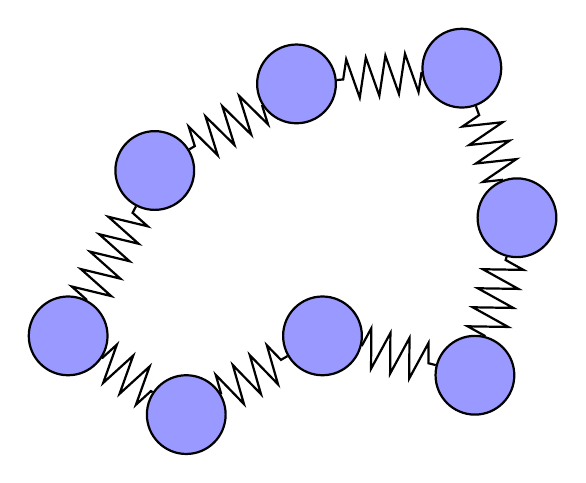
\begin{tikzpicture}
\node[circle,fill=blue!40!white,draw, minimum size=1.0cm, thick, font=\boldmath] (A) at  (0.5,1) {};
\node[circle,fill=blue!40!white, draw, minimum size=1.0cm, thick] (B) at  (2,0)  {};
\node[circle,fill=blue!40!white, draw, minimum size=1.0cm, thick] (C) at  (3.73,1)  {};
\node[circle,fill=blue!40!white, draw, minimum size=1.0cm, thick, font=\boldmath] (D) at  (5.666,0.5) {};
\node[circle,fill=blue!40!white, draw, minimum size=1.0cm, thick] (E) at  (6.2,2.5)  {};
\node[circle,fill=blue!40!white, draw, minimum size=1.0cm, thick] (F) at  (5.5,4.4)  {};
\node[circle,fill=blue!40!white, draw, minimum size=1.0cm, thick] (G) at  (3.4,4.2)  {};
\node[circle,fill=blue!40!white, draw, minimum size=1.0cm, thick] (H) at  (1.6,3.1)  {};

\draw[decorate,decoration={zigzag,segment length=2.5mm, amplitude=2.5mm}, thick] (A) -- (B);
\draw[decorate,decoration={zigzag,segment length=2.5mm, amplitude=2.5mm}, thick] (B) -- (C);
\draw[decorate,decoration={zigzag,segment length=2.5mm, amplitude=2.5mm}, thick] (C) -- (D);
\draw[decorate,decoration={zigzag,segment length=2.5mm, amplitude=2.5mm}, thick] (D) -- (E);
\draw[decorate,decoration={zigzag,segment length=2.5mm, amplitude=2.5mm}, thick] (E) -- (F);
\draw[decorate,decoration={zigzag,segment length=2.5mm, amplitude=2.5mm}, thick] (F) -- (G);
\draw[decorate,decoration={zigzag,segment length=2.5mm, amplitude=2.5mm}, thick] (G) -- (H);
\draw[decorate,decoration={zigzag,segment length=2.5mm, amplitude=2.5mm}, thick] (A) -- (H);
\end{tikzpicture}
\end{document} 
